\section{Durchführung und Aufbau}
\label{sec:Durchführung}
Als erstes wird die Strecke $L$ zwischen Photoelektrode und Spalt, wie in Abbildung \ref{fig:aufbau} zu sehen ist, vermessen.
\begin{figure}
  \centering
  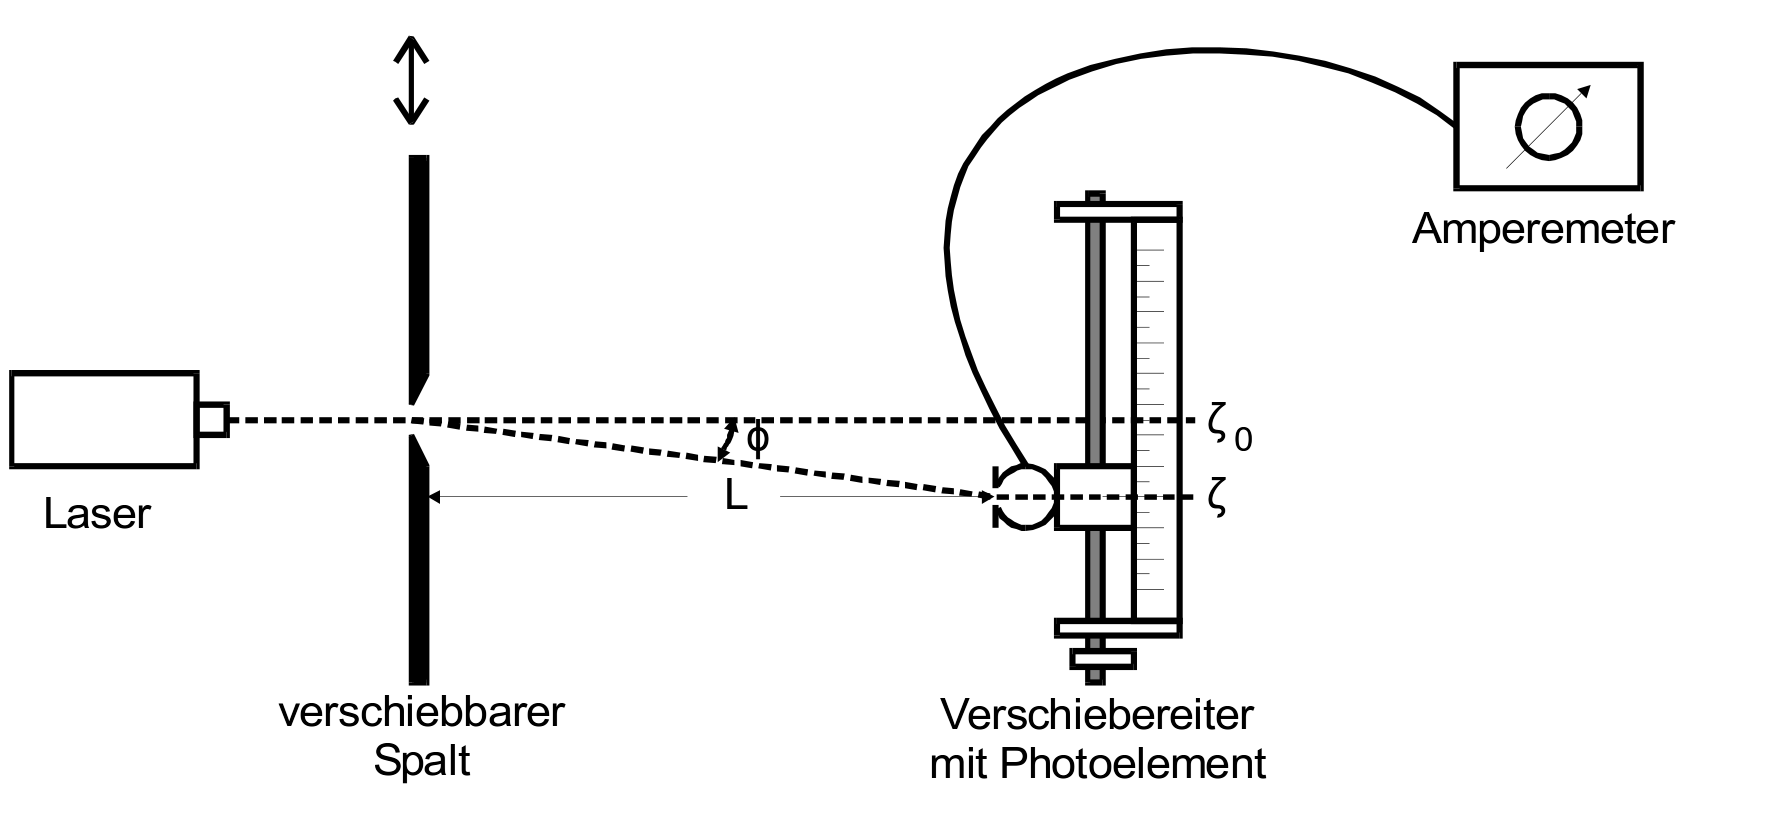
\includegraphics[height=5cm]{picture/Aufbau.png}
  \caption{Versuchsaufbau}
  \label{fig:aufbau}
\end{figure}
Anschließend wird einmal der Dunkelstrom $I_\text{D}$ der Photodiode gemessen. Dann kann nach dem Einspannen des Spaltes in die dafür vorgesehene Messaperatur der Laser eingeschaltet werden und das Beugungsbild vermessen werden. Dazu wird zunächst das Hauptmaxima ermittelt und von diesem ausgehend zu beiden Seiten 25 Messwerte genommen. Dies geschieht indem die Fotodiode jeweils um 1mm auf der Schiene vom Hauptmaximum entfernt wird und der Fotostrom $I$ ausgemessen wird.
Nachdem das Beugungsbild vermessen ist, wird anschließend die Spaltbreite an einem Mikroskop vermessen. Dafür wird zunächst der Maßstab anhand eines geeigneten Referenzobjekt ermittelt und mit Hilfe diesem, die Spaltbreite $b$ des Spalts ausgerechnet. Der Versuch ist für alle 3 Einzelspalte als auch für den Doppelspalt durchzuführen.
